\documentclass[superscriptaddress, twocolumn, prl]{revtex4}

\usepackage{amsmath}    % need for subequations
\usepackage[pdftex]{graphicx}   % need for figures
\usepackage{verbatim}   % useful for program listings
\usepackage{color}      % use if color is used in text
\usepackage{subfigure}  % use for side-by-side figures
\usepackage{hyperref}   % use for hypertext links, including those to external documents and URLs
\allowdisplaybreaks

\begin{document}

\title{Towards an Understanding of the Aerodynamic Origin of Rodent Ultrasonic Vocalizations}

\author{Matthew Dornfeld}
\affiliation{Laboratory of Mathematical Physics, Rockefeller University, 1230 York Ave, New York, NY 10065, USA}

\author{Diego Laplagne}
\affiliation{
Brain Institute, Federal University of Rio Grande do Norte, Av. Nascimento de Castro 2155, Natal, RN, 59056-450, Brazil}

\author{Martin Elias Costa} 
\affiliation{Physics Department, FCEN, UBA Ciudad Universitaria, Pab. 1 (1428), Buenos Aires, Argentina}

\author{Marcelo Magnasco}
\affiliation{Laboratory of Mathematical Physics, Rockefeller University, 1230 York Ave, New York, NY 10065, USA}
\date{\today}
\begin{abstract}
We investigate the physical production mechanism behind mammalian narrowband ultrasonic vocalizations, using Long Evans rats as a model organism. We develop a curve fitting algorithm that extracts discontinuous jumps in frequency from many recorded calls ($n=9589$) from several rats ($N=11$). We also develop a clustering algorithm that fits this data to a aerodynamic oscillator model. Our results support the previously suggested hypothesis that rat ultrasonic vocalizations are not the result of vibrating vocal folds but are in fact generated by an aerodynamic oscillator. This aerodynamic oscillator was previously suggested to be a hole tone whistle. However, our results are inconsistent with this conjecture. We conclude that a more complete aerodynamic oscillator model would have to take into account the resonance frequencies of the rat vocal tract.   
\end{abstract}
\maketitle
Although the purposes of animal vocalizations are numerous, the apparatus by which they are produced seems to be largely conserved across mammalian and bird species. This apparatus consists of membranous vocal fold tissues stretched across the larynx (or syrinx in birds). This tissue attaches to laryngeal muscles, which can alter its tension and degree of adduction. When air is forced past them, by the lungs, the vocal folds oscillate and emit audible sounds, the frequency of which are determined by the vocal fold tension \cite{Berke2010}. Across species, the fundamental frequencies $f$ of audible mammalian vocalizations, which span several orders of magnitude in mass, approximately obey a power law of the form $f\propto M^{-\alpha}$, where M is the species mass \cite{Fletcher2010}. However, many species of the orders Rodentia and Cetacia are known to produce narrowband ultrasonic whistles and broadband ultrasonic clicks, in addition to their sonic vocalizations \cite{white1998,berry1970natural,Fenton1998,Jones2006,bogdanowicz1994,Frankel2009,Whitehead2009,Rendell1999,Kastelein2000,Jefferson1993}. While the sonic vocalizations obey the aforementioned scaling law well, ultrasonic calls from the same species completely diverge from the power law fit by over an order of magnitude (see Fig. \ref{fig:frequency_scaling}). There is currently some debate over the exact nature of these ultrasonic calls, and the divergence from the scaling law is indicative that the production mechanism is fundamentally different from that of audible vocalizations.

Of the above mentioned ultrasonic vocalizations (USVs), the broadband clicks are believed to serve noncommunicative echolocative purposes. In odontocetes, the broadband clicks are known to be produced by a structure, called the phonic lips, which strike the fatty tissue of a structure called the melon, which transmits the vibrations to the surrounding water. However, the production mechanism behind narrowband calls in cetaceans is currently unknown. Furthermore, they are believed to be directed to conspecifics for the purpose of communication. Thus, the study of these vocalizations has broader implications for the fields of animal communication and ethology as a whole \cite{Reidenberg2010}. Rats exclusively exhibit narrowband type USVs, and there has been some experimental work that discounts the possibility narrowband calls are produced by vibrating vocal folds. Work done by Roberts and Riede showed an increase in the fundamental frequency of rat USVs, when they replaced the air in the rat vocal tract with heliox gas. This is inconsistent with a vibrating vocal fold model, since the fundamental frequency would be set by the mechanical oscillations \cite{Roberts1975, Riede2011}. Further work by Sanders consisted of inserting a camera into the upper vocal tract of anesthetized rats. The vocal folds were observed to remain tense and did not oscillate when a USV was elicited through brain stem stimulation \cite{Brudzynski2010}. Although previous work indicates the source of rat USVs are aerodynamic oscillations, as opposed to mechanical ones, the structure of this aerodynamic oscillator is still unclear. This paper attempts to determine the specific nature of the oscillator by extracting features from rat USVs and fitting them to an aerodynamic oscillator equation. Our results should be directly applicable to other rodents, such as mice, which exhibit narrowband USVs. In addition, we hope they also provide insight into the production mechanism behind narrowband USVs in cetacean species. 

\begin{figure}[!ht]
\centering
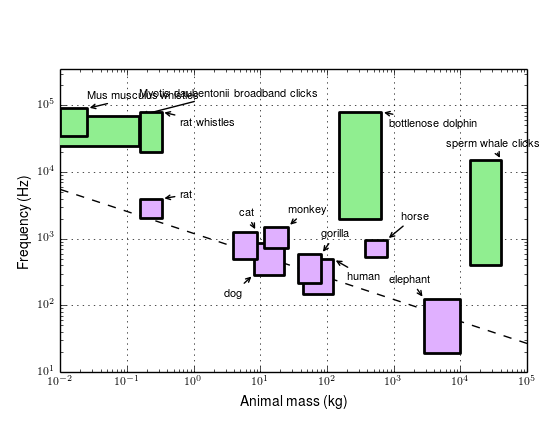
\includegraphics[width=\columnwidth]{frequency_scaling.png}
\caption{\label{fig:frequency_scaling} The purple boxes show the ranges of audible frequencies emitted by several mammals plotted against the ranges of their masses. The solid and dotted lines show plots of a frequency scaling law of the form $f\propto M^{-\alpha}$. The dotted line ($\alpha=\frac{1}{3}$) is a theoretical relationship based on the conjecture that the average frequency emitted in audible vocalizations should be inversely proportional to the linear scale of the animal. The solid line ($\alpha=0.4$) is a power law fit to the purple boxes \cite{Brudzynski2010}. The green boxes show the range of ultrasonic frequencies emitted by several mammalian species plotted against their masses \cite{Fletcher2010, white1998,berry1970natural,Fenton1998,Jones2006,bogdanowicz1994,Frankel2009,Whitehead2009,Rendell1999,Kastelein2000,Jefferson1993}.}
\end{figure}
In general, an aerodynamic whistle results when a mean airflow impinges on or grazes a sharp edge. At high enough Reynolds numbers ($Re>1000$) boundary layer separation occurs. An air jet, which supports small velocity perturbations, is formed. The geometry of the jet determines the perturbation frequencies, which are amplified \cite{Batchelor1962}. The amplified disturbances are a source of sound, radiating acoustic energy into the farfield. On its own boundary layer separation at an edge is a very inefficient mechanism for sound production. This can be remedied by using the flow separated jet to drive an acoustic resonator. This is the mechanism behind many air driven musical instruments, such as flutes and organ pipes. Perturbations in the separated flow act as a nonlinear driving force, creating an acoustic response in the resonator. The acoustic flow in the resonator then further excites perturbations in the separated flow. This creates a positive feedback mechanism, which amplifies a preferred frequency of the system \cite{Fletcher1998}. At higher amplitudes the perturbations in the separated flow can destabilize into a vortex street. The oscillation condition for the acoustic system can be determined in a number of ways. A spatial normal mode analysis can be used to convert the wave equation to a nonlinear time domain ODE. This equation is then linearized and a feedback condition is enforced \cite{Auvray2012, Auvray2014}. Other methods involve neglecting the complicated destabilization process and assuming the existence of a fully formed vortex street , and calculating the velocity induced by the interaction of the vortex street with the downstream structure. The phase of the induced velocity is then matched to that of the perturbations in the boundary separated flow to ensure the positive feedback mechanism. In general the oscillation condition has the form
\begin{equation}
\label{eq:whistle}
\frac{fL}{U_{c}}=n-\gamma,
\end{equation}
where $f$ is the tonal frequency emitted in the acoustic far field, $L$ is a characteristic length scale of the system, $U_c$ is the convection velocity of the boundary layer perturbations, $n$ is the acoustic mode number, and $\gamma$ is a constant that is dependent on the type of oscillator. The quantity, $\frac{U_c}{f}$ is the spacing between successive peaks of the boundary layer disturbances, thus $n-\gamma$ has the physical interpretation of being the number of disturbance wavelengths (or number of discrete vortices) that can fit in the length $L$. Discontinuous jumps in the acoustic frequency $f$ can occur. This is due to a change in stability of the underlying flow of the oscillator, caused by bifurcations in the time domain ODE, and corresponds to a unity increase or decrease in the mode number $n$. Fig. \ref{fig:specgram} shows examples of two frequency jumps in a rat whistle \cite{Howe2008,Blake1986}.

It is currently unclear how rat anatomical structures would operate together as an aerodynamic oscillator. Fig. \ref{fig:gamma_error} shows $\gamma$ for several different types of oscillator mechanisms that can possibly correspond to rat anatomy. Below we will discuss how to fit data extracted from recordings of rat vocalizations to Eq. \ref{eq:whistle} to get a determination of $\gamma$, but first we will discuss how different types of oscillators may correspond to rat anatomy. As a starting point we can consider the doubly open pipe resonator as a naive model for the upper vocal tract. The resonance frequencies of this system are given by Eq. \ref{eq:whistle} with $\gamma=0$. When an anatomically realistic value of $L$ is used (about 1.5 cm), the resonance frequencies given by this equation are similar to those seen in rat USV recordings. This indicates the resonance frequencies of the vocal tract will be an important feature of an accurate model for USV production. However, by only considering the passive resonance frequencies we neglect any transient behavior, such as frequency jumps, seen in USV recordings. A more complete theory would take into account the nonlinear transient behavior of the jet driving force emerging from the vocal folds. Several mean flow driven oscillators have been investigated in the past. We now overview some of the more well known ones.

For the rat phonatory system to operate as an edge tone, the vocal folds would focus air coming up from the lungs into a plane jet which impinges on an edge like downstream structure- the most likely candidate for which is the junction between the nasal and buccal cavities. A K\'{a}rm\'{a}n vortex street is then shed antisymmetrically into the nasal and buccal cavities \cite{Holger1977,Howe2008}. However, if this were the mechanism, it would be expected that sound is emitted equally from both the nose and the mouth, and it has been observed that sound is primarily emitted from the mouth. In addition, the hole formed by the vocal folds has been observed, in anesthetized rats, by camera, to be approximately circular in shape throughout vocalization. This precludes the possibility of them focusing the stream of air into a plane jet \cite{Brudzynski2010}.  

It is also possible, air emerging from the vocal folds flows over the junction to the nasal cavity into the buccal cavity, acting as a cavity resonator. Vortices are shed at the leading edge of the opening to the nasal cavity and interact with the cavity and trailing edge to induce a velocity that radiates sound into the far field and provides acoustic feedback to reinforce vortex production at the leading edge. The analysis of cavity resonators, and thus the value of $\gamma$, depends on the ratio of the width of the cavity opening to its depth. If this ratio is less than unity, the cavity is considered shallow, and the energy stored in the cavity can be neglected. However, if the ratio is greater than unity, the cavity is considered deep, and this energy must be considered. The length of the nasal cavity is much greater than the width of the entrance to the nasal cavity at the nasal-bucaal junction. Thus, the deep cavity model seems to correspond better to rat anatomy. However, for completeness we include both values of $\gamma$ in Fig. \ref{fig:gamma_error} \cite{Howe2008, Brudzynski2010}.

Roberts \cite{Roberts1975}, Brudzynski, and Fletcher \cite{Brudzynski2010} suggested the hole tone to be the most biologically realistic model for rat USV production. It consists of a circular jet impinging on a downstream aperture of slightly greater width. In this model, the vocal folds focus the air from lungs into a circular jet. The most likely anatomical structures for the downstream aperture are either the space between the base of the tongue and the soft palate or the one between the epiglottis and the cranial wall of the oropharynx. Disturbances are amplified as they are convected along with the mean flow of the jet and are the source of a fluctuating flow into the downstream aperture. The flow through the aperture generates acoustic radiation, which is the source of sound in the farfield and feedback in the form of additional disturbance energy for the jet. Roberts constructed an artificial hole tone, consisting of axially aligned circular apertures in two metal plates. He was able to reproduce sounds resembling rat USVs with physiologically realistic blowing pressure. This model is problematic because an anatomical structure corresponding to the downstream aperture has not been reliably identified. In addition, it does not take into account the resonant properties of the rat vocal tract. The value of $\gamma$ in Fig. \ref{fig:gamma_error} was obtained experimentally as well as theoretically under the condition that the length between the apertures is much greater than the radius of the jet. A fact that will become important in our analysis later is this condition is not necessarily met in the rat vocal tract as the radius of the opening in the vocal folds during vocalization as well as the distance between the apertures are both on the order of 1 mm \cite{Brudzynski2010,Chanaud1965,Howe2008}.

To fit data to this model, we examined the frequency jump points from many recorded calls ($n=9589$) from eleven different Long-Evans rats (nine males and two females). These recordings were obtained by sampling calls at 250-300 kHz using a condenser ultrasound Avisoft-Bioacoustics CM16/CMPA-5V microphone connected to a National Instruments data acquisition card. The recordings were then divided into call snippets based on quiescence times greater than 20 ms between vocalizations. Afterwards, the reassigned spectrogram of each call snippet was computed \cite{Gardner2006}. Since each vocalization is largely monotonal, a curve can be fitted to the call in time-frequency space by finding the frequency with the most power and computing the average of the seven frequency points surrounding and including that maximum- weighted by the amount of power in each frequency (see Fig. \ref{fig:specgram}).This is done for each time point. Jump points can then be determined by finding points where the curve rapidly changes value. For each jump point, the after frequency can be plotted against the before. The data naturally groups itself into clusters along straight lines. In doing so, we have extracted features with drastically lower dimensionality than the original data, and we hypothesize that each cluster corresponds to one type of mode transition, with $n\rightarrow n\pm1$. 
\begin{figure}[!ht]
\centering
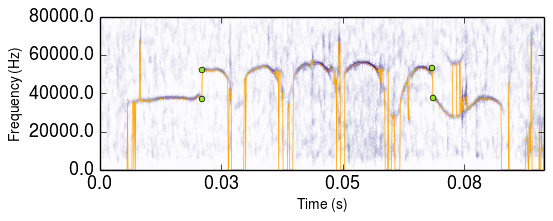
\includegraphics[width=\columnwidth]{specgram.png}
\caption{\label{fig:specgram} Reassigned spectrogram of a segment of a rat USV. The orange line is the output of the curve fitting algorithm. The green circles show the output of the jump extraction algorithm.}
\end{figure}
To fit the extracted jump points to Eq. \ref{eq:whistle} we developed a clustering algorithm, which as input, accepts a list of slopes of straight lines. The number of clusters in the output is equal to the length of the list. The algorithm then iterates over each jump point in the dataset and computes the perpendicular distance of the point to the line defined by each slope. The point is then assigned to the line for which this value is minimum. If $\left(f_{1},\: f_{2}\right)$ and $\left(n,\: n\pm1\right)$ are the frequencies and mode numbers before and after a jump respectively, by dividing the after jump frequency mode relation by the before jump relation, we get 
\begin{equation}
\label{eq:freqmode2}
\frac{f_{2}}{f_{1}}=m(c,\gamma)=\frac{n\pm1-\gamma}{n-\gamma},
\end{equation}where $c$ is the cluster to which that jump has been assigned, and $\left(n,\: n\pm1\right)$ is a function of the cluster. Several mode transitions were experimented with to best fit the data. In the extracted jumps, we found transitions in mode numbers ranging from $n=2$ to $n=6$. The $n=1$ mode seems to correspond to 22-kHz alarm calls, which do not exhibit jumps as often and therefore are not represented in our dataset. Not all rats in our study produced enough jumps in all mode regions to fit the data to our algorithm, so underpopulated modes were excluded for some rats. Eq. \ref{eq:freqmode2} can then be used to generate the slopes needed as input for the algorithm. We can define a cost function $C\left(\gamma \right)$ that is the sum of squares of the perpendicular distances of each point to their assigned line \cite{jump_appendix}. By minimizing $C\left(\gamma \right)$, we can get a determination for which cluster each point belongs to as well as a numerical calculation for the value $\gamma$. 
\begin{figure}[!ht]
\centering
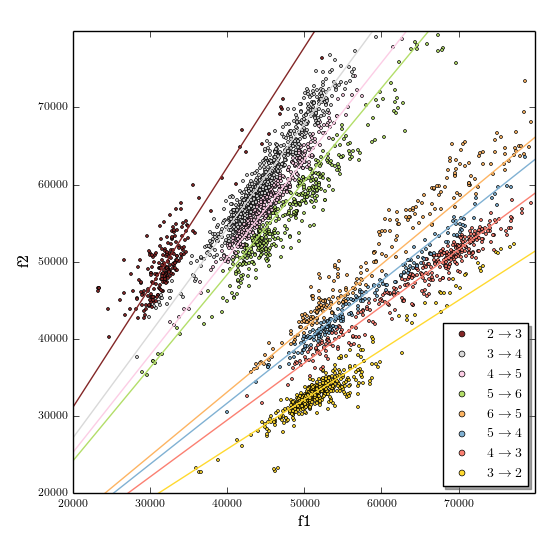
\includegraphics[width=\columnwidth]{V4.png}
\caption{\label{fig:jumps}After jump frequency plotted against before jump frequency for jumps extracted from V4. The points are color coded according to the transition cluster they were assigned by the clustering algorithm. The legend in the bottom right shows which mode transitions ($n\rightarrow n\pm1$) correspond to the color. The lines are plots of Eq. \ref{eq:freqmode2}, for $\gamma=\gamma_{min}^{V4}$ and obey the same color coding scheme.} 
\end{figure}

Fig. \ref{fig:jumps} shows the output of the clustering algorithm for rat V4 for $\gamma=\gamma_{min}^{V4}$, the value that minimize $C\left(\gamma \right)$. Also shown are plots of the lines defined by $m\left(c,\gamma_{min}^{V4}\right)$, for each mode transition cluster. We also experimented with adding a parameter that offsets the lines defined by Eq. \ref{eq:freqmode2} from the origin. As expected, in all cases, it was found to be effectively zero, so we do not include it in further analysis. The data in Fig. \ref{fig:jumps} is grouped into eight clusters. Four correspond to up transitions and four correspond to down transitions. Unlike some other rats used in this study, V4 exhibits a significant number of jump points in the $2\rightarrow3$ and $3\rightarrow2$ transition clusters, which are mostly populated by jumps between constant frequency segments in the 30 kHz range to constant frequency segments in the 50 kHz and vice versa, which are rarely observed in recordings \cite{Wright2010}. These clusters are noticeably distinct from the others and can be separated out by visual inspection. The clusters that represent transitions between higher regions present more of an overlap with each other. The $3\rightarrow4$, $5\rightarrow6$, $4\rightarrow3$, and $6\rightarrow5$ clusters show clear drop offs in density at their borders, which seems to be well represented in the output of the algorithm. However, the $4\rightarrow5$ and $5\rightarrow4$ transition clusters do not seem to be well represented in the data for this rat. Thus, it is hard to identify these clusters based on visual inspection of the density of jump points, although we still believe them to be present in smaller numbers. It is also worth noting that, removing those clusters from the algorithm did not produce a significant change in the calculated value of $\gamma$. 
\begin{figure}[!ht]
\centering
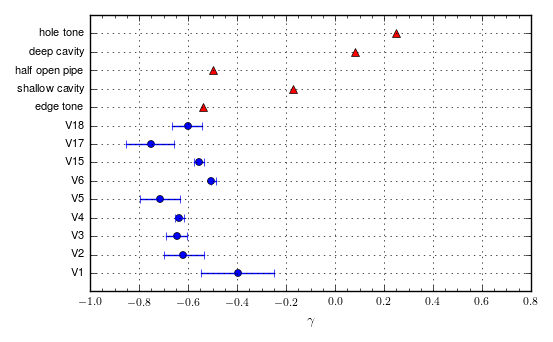
\includegraphics[width=\columnwidth]{theta_error_minus.png}
\caption{\label{fig:gamma_error} The blue shows $\gamma_{min}^{rat}$ along with 95 \% confidence intervals obtained from bootstrap analysis. The red shows values of $\gamma$ known for several aerodynamic oscillators \cite{Howe2008}.}
\end{figure}

The results of Figs. \ref{fig:jumps} and \ref{fig:gamma_error} give clear indications about the nature of the oscillator mechanism underlying narrowband USVs. Upon inspection of Fig.\ref{fig:jumps} evidence of hysteresis can be seen as the densities of opposite transition clusters are not mirror images of each other and seem to be translated and warped along the lines with slope $m\left(c,\gamma_{min}^{rat}\right)$, which would be expected for an aerodynamic oscillator. Furthermore, the points of each cluster seem to be distributed roughly symmetrically around these lines. This indicates the frequency jumps are the result of a noisy process in the vicinity of a critical point of the system, which would also be expected for an aerodynamic oscillator. Fig. \ref{fig:gamma_error} shows a comparison of the values of $\gamma_{min}$ obtained for the rats used in this study with ones known for different aerodynamic oscillators. Based on these results, we can conclusively rule out the edge tone, shallow cavity, and deep cavity mechanisms as being the source of rat USVs. Furthermore, as expected, the jumps cannot simply be explained by transitions between the passive resonance frequencies of an open pipe. The values of $\gamma$ obtained from this study somewhat correspond with the one known for the hole tone. However, the correspondence is not exact. Thus, we conclude from this study rat USVs cannot be fully explained by the hole tone model. Although the it accurately accounts for the axisymmetric jet driving force, we believe the reason for the discrepancy is it does not take into the resonance frequencies of the rat vocal tract. We believe a more accurate model would consist of treating the upper vocal tract as a linear resonator being excited by an axisymmetric jet driving force. Unfortunately, a complete theory of an nonlinear axisymmetrically driven resonator does not exist. Current work by our group is focused on developing a more complete theory of this model and of the hole tone so a more detailed comparison can be made.

\bibliographystyle{prsty}
\bibliography{mdornfe1.bib}

\begin{acknowledgments}
DL and MEC would like to acknowledge funding from the Leon Levy Foundation. MEC would like to acknowledge funding from CONICET and the Fulbright Foundation.
\end{acknowledgments}
\end{document}